\documentclass[a4paper, 12pt]{article}
\usepackage[english]{babel}
\usepackage[utf8]{inputenc}
\usepackage[T1]{fontenc}
\usepackage{lmodern}
\usepackage{hyperref}
\usepackage[numbers, sort&compress]{natbib}
\usepackage{calc}
\usepackage{fancyhdr}
\usepackage{graphics}
\usepackage{nowidow}
\usepackage{color}
\usepackage{subcaption}
\usepackage{epsfig}
\usepackage{epstopdf}


\newlength{\eqMargin}
\newlength{\eqHorizMargin}
\newlength{\eqVertMargin}

\setlength{\eqMargin}{20mm}
\setlength{\eqHorizMargin}{\eqMargin}
\setlength{\eqVertMargin}{\eqMargin}

% Paper
\setlength{\paperwidth}{210mm}
\setlength{\paperheight}{297mm}

% Rid the extra space
\setlength{\hoffset}{-1in}
\setlength{\voffset}{-1in}
\addtolength{\hoffset}{\eqHorizMargin}
\addtolength{\voffset}{\eqVertMargin}

% Set margin from the page border (horizontal)
\setlength{\oddsidemargin}{0pt}
\setlength{\evensidemargin}{0pt}

% Header
\setlength{\topmargin}{0pt}
\setlength{\headheight}{30pt}
\setlength{\headsep}{18pt}
\renewcommand{\headrulewidth}{0pt}

% Footer
\addtolength{\footskip}{18pt}
\renewcommand{\footrulewidth}{0pt}

% Margin notes
\setlength{\marginparsep}{0pt}
\setlength{\marginparwidth}{0pt}

% Text
\setlength{\textwidth}{\paperwidth - \hoffset - \hoffset - 25.4mm - 25.4mm}
\setlength{\textheight}{\paperheight - \voffset - \topmargin - \headheight - \headsep - \footskip - \voffset - 25.4mm - 25.4mm}

%\setlength{\labelwidth}{20mm}

% Hyperref settings
\hypersetup{
    unicode=true,					% non-Latin characters in Acrobat's bookmarks
    pdftoolbar=true,				% show Acrobat's toolbar?
    pdfmenubar=true,				% show Acrobat's menu?
    pdffitwindow=false,				% window fit to page when opened
    pdfstartview={FitH},			% fits the width of the page to the window
    pdftitle={S-26.3120 Radio Engineering, laboratory course},	% title
    pdfauthor={Tuomas Leinonen} {Sampo Salo},	% author
    pdfsubject={Radio Engineering},	% subject of the document
    pdfcreator={LaTeX},				% creator of the document
    pdfproducer={Aalto},			% producer of the document
    pdfkeywords={radio} {gsm} {bs} {tx},	% list of keywords
    pdfnewwindow=true,				% links in new window
    colorlinks=true,				% false: boxed links; true: colored links
    linkcolor=black,				% color of internal links
    citecolor=black,				% color of links to bibliography
    filecolor=black,				% color of file links
    urlcolor=black					% color of external links
}

% Bad hyphenation
%\hyphenation{}

\definecolor{dkred}{rgb}{0.6, 0, 0}
\definecolor{dkgrn}{rgb}{0, 0.6, 0}
\definecolor{dkblue}{rgb}{0, 0, 0.6}

\pagestyle{fancy}
\lhead{S-26.3120 Radio Engineering, laboratory course\\Lab 1: GSM BS TX -- Final report}
\rhead{Sampo Salo, 79543L\\Tuomas Leinonen, 84695P}
\cfoot{\thepage}


\begin{document}

\begin{titlepage}
\pagestyle{empty}
\begin{center}

\vspace*{3cm}
\noindent\LARGE{\textbf{S-26.3120 Radio Engineering, laboratory course}}

\vspace*{2cm}

\Large{\textbf{Lab 1: GSM Base station Transmitter}}\\

\vspace*{1.5cm}

\large{\textbf{Final report}}\\
\vspace{1.5cm}
\large{\today}
	
\vspace*{3cm}
\large{
	\begin{tabular}{l l}
		\textbf{Group 4:} 	& \\
		Sampo Salo			& 79543L	\\
		Tuomas Leinonen 	& 84695P		
	\end{tabular}
}

\end{center}

\end{titlepage}


\section{Introduction}

The first laboratory assignment was mainly about learning to use the radio
frequency measurement devices. The devices included a signal source, spectrum
analyzer, and a vector network analyzer. The measurement setup included also
cables, attenuators, and connectors. The signal source was actually a GSM
base station (BS) transmitter (see Fig. \ref{fig:bs}), and the assignment simulated 
measurements one could face in real life as well. 

\begin{figure}[h!]
	\begin{center}
	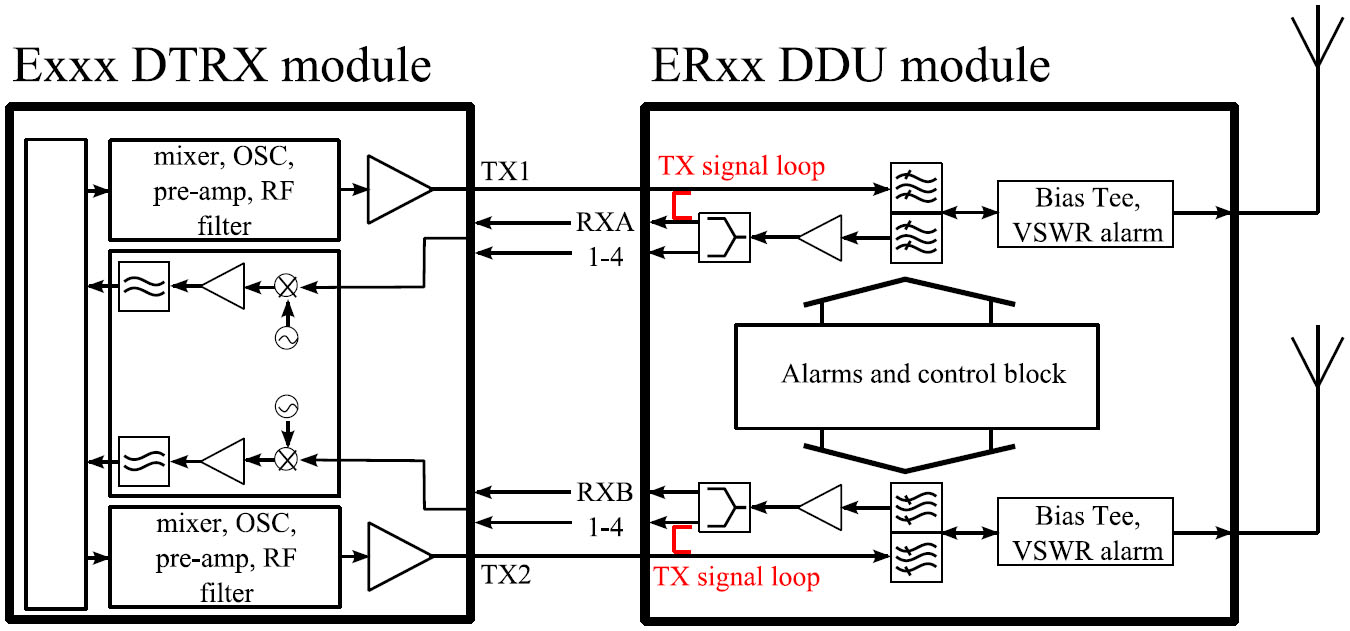
\epsfig{file=img/bs.jpg, width=\textwidth}
	\caption{GSM base station block diagram.}
	\label{fig:bs}
	\end{center}
	\vspace*{-12pt}
\end{figure}

The assignment consisted of four different tasks. In the first task, the base station 
transmitter (TX) output power was measured using five different output power levels. 
The base station's dynamic power control allowed the downlink power to be reduced in 
15 steps with a step size of 2 dB. In the second and third tasks the base station 
performance was compared to GSM specifications. The purpose of the second task 
was to verify that the in-band output spectrum does not exceed the system specific 
levels for an individual transceiver. The third task covered the whole measurable 
frequency band, as the GSM specifications set interference limits for out-of-band 
frequencies as well. In the last task, the diplexer insertion loss was measured.

This report is divided in five sections. The first section after Introduction describes 
the general measurement procedures for the measurement setups used. The third section 
presents the measurement results and error estimates, while the fourth section 
states the conclusions. In the final section, feedback is given to further improve 
the first laboratory assignment of the course.


\newpage
\section{Measurement steps}

There were two types of measurements; power measurements with a spectrum analyzer 
(SA) and two-port measurements with a vector network analyzer (VNA). While the 
first three measurement tasks (i.e., $3.1 - 3.3$) were of the first kind, the 
last measurement (i.e., 3.4) was carried out using a VNA. The aforementioned 
measurement setups are described in detail in the following subsections, respectively. 
The setups correspond very closely to those presented in the pre-study.


\subsection{Spectrum analyzer measurements}

Spectrum analyzer measurements will be carried out as the following figure 
(Fig. \ref{fig:sa}) suggests. A laptop running maintenance software is controlling 
the base station which is in turn connected to the \textit{HP 8596E} spectrum 
analyzer as follows. The antenna connector of the A-half is connected via a 
SMA-cable to chain of attenuators with nominal attenuations of 6 dB, 10 dB, 
and 20 dB, respectively (i.e., 36 dB in total). Following the attenuator 
chain is a N-type cable connected to the SA.

\begin{figure}[h!]
	\begin{center}
	\epsfig{file=img/sa.jpg, width=\textwidth}
	\setlength{\unitlength}{1mm}
	\begin{picture}(1, 1)
		\put(-60, 95){\makebox(0,0){Laptop running}}
		\put(-60, 90){\makebox(0,0){maintenance}}
		\put(-60, 85){\makebox(0,0){software}}
		\put(-67, 48){\makebox(0,0){\textcolor{white}{BS: ANT$_\mathrm{A}$}}}
		\put(-30, 47){\makebox(0,0){\textcolor{white}{SMA-cable}}}
		\put(20, 71){\makebox(0,0){Attenuators:}}
		\put(22.3, 66){\makebox(0,0){$6 + 10 + 20$ dB}}
		\put(67, 55){\makebox(0,0){N-cable}}
		\put(10, 10){\makebox(0,0){HP 8596E SA}}
	\end{picture}
	\vspace*{-12pt}
	\caption{Measurement setup used in spectrum analyzer measurements: 
	BS: ANT$_\mathrm{A}$ $\rightarrow$ SMA-cable $\rightarrow$ $6 + 10 + 20$ dB attenuators $\rightarrow$ N-cable $\rightarrow$ HP 8596E SA}
	\label{fig:sa}
	\end{center}
	\vspace*{-12pt}
\end{figure}

For all the SA measurements, following settings were used: zero span, 
video and resolution bandwidth of 30 kHz, 500-measurements averaging 
and10 dB input attenuation. Changing the center frequency, we could 
read the required power levels using markers. The SA was not explicitly 
calibrated as the assistant deemed it unnecessary. Also, required 
connectors/adapters were not available.

In the \textit{2G Flexi BTS Site Manager (Flexi EDGE) EX4\_0 Build 058} 
(supplied by Nokia Siemens Networks) maintenance software (SW), 
\textit{BCCH Transmission Test} was used throughout the measurement. 
Test parameters are listed in the following table (Table \ref{tbl:bcch}). 

\begin{table}[!h]
	\begin{center}
	\caption{Used \textit{BCCH Transmission Test} parameters.}
	\label{tbl:bcch}
	\renewcommand*{\arraystretch}{1.2}
	\begin{tabular}{lcl}
	\textbf{Option} 		& \textbf{Value} 	& \textbf{Note} \\
	\hline
	TRX Number				& TRX 1				& A-half (ANT$_\mathrm{A}$ is used as BS output) \\
	Power					& 0					& also levels 1, 7, 14 and 15 for the first measurement \\
	ARFN					& 0					& $f_\mathrm{RX} = 890$ MHz and $f_\mathrm{TX} = 935$ MHz \\
	Network Color Code		& 0					& \\
	Base Station Color Code & 0					&
	\end{tabular}
	\end{center}
	\vspace*{-12pt}
\end{table}

For the first measurement (\textit{Dynamic Downlink Power Control Level}), 
the spectrum analyzer is tuned to 935 MHz while the \textit{Power} parameter 
is changed (values 0, 1, 7, 14 and 15 are used) in the control software. 
The power level is written down.

For the second measurement (\textit{In-band output spectrum}), the TX power 
is reset to its maximum value (i.e., \textit{Power} is set to 0 in the SW).
The power is measured like before, but now the frequency is offset to test 
for a spectral mask. The following positive frequency offsets (based on the 
GSM standard) are used: 100, 200, 250, 400, 600, 800, 1000 and 1200 kHz.

In the final SA measurement (\textit{Interference}), we scan both the lower 
and upper bands ($100 \mathrm{\;kHz} - 1 \mathrm{\;GHz}$ and $1 - 12.75$ GHz, 
respectively) for the single, most powerful spurious emission. The lower limit
of the lower band was originally 9 kHz in the instructions, but was increased 
to 100 kHz due to limitations in the SA. Maximum TX power is used.


\subsection{Measurements with the vector network analyzer}

The last measurement was carried out using a \textit{Rohde \& Schwarz ZVL} VNA, 
calibrated by the assistant prior to our arrival. The calibration settings were 
as follows: full two-port calibration with 1577 points within the $850 - 1000$ 
MHz band, $-20$ dBm transmit power, and an averaging factor of 100. The SMA-cables
with a copper colored jacket were included in the calibration (see Fig. \ref{fig:vna}).

\begin{figure}[h!]
	\begin{center}
	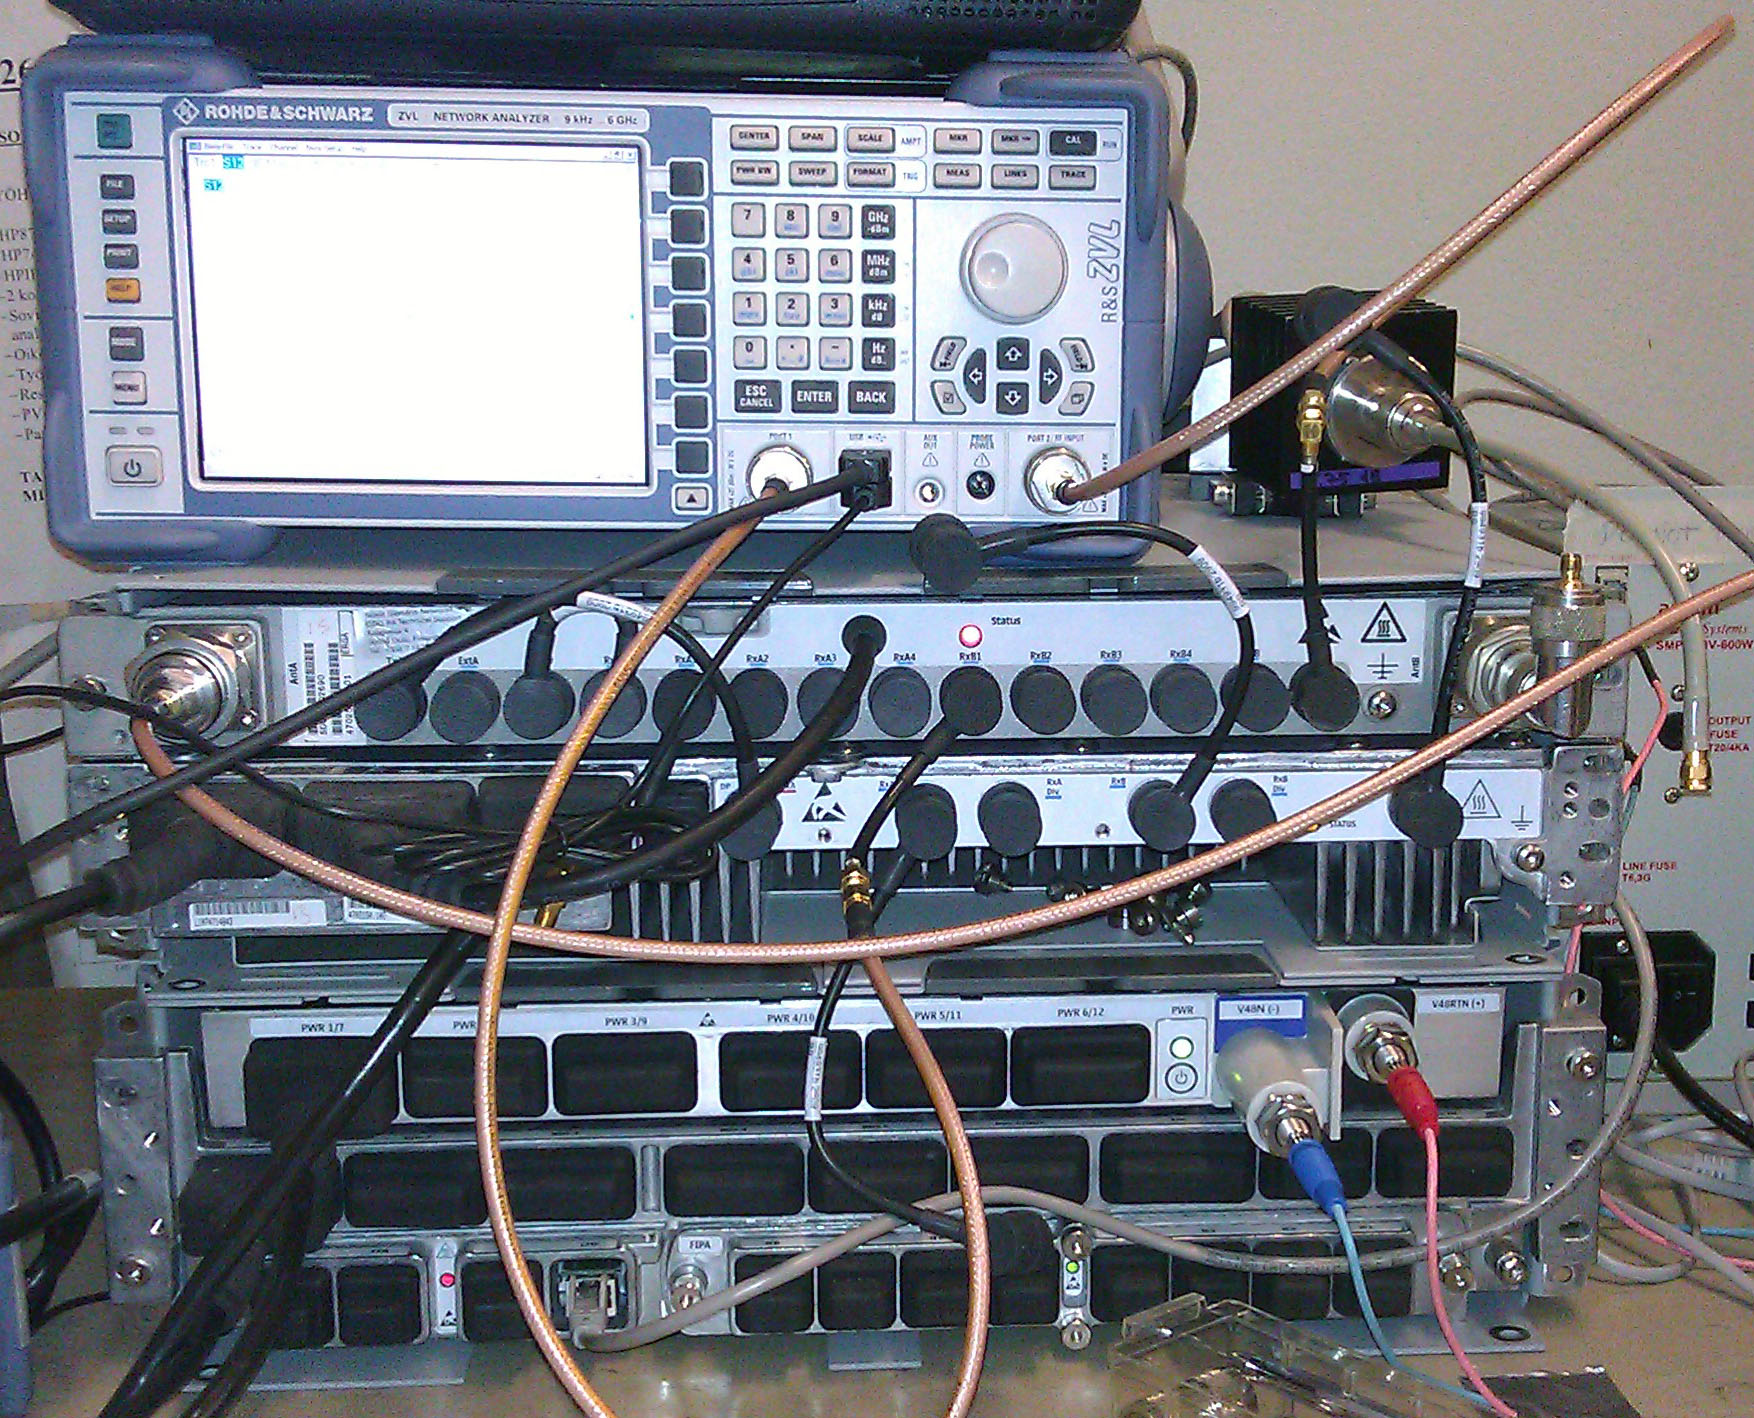
\epsfig{file=img/vna.jpg, width=\textwidth}
	\setlength{\unitlength}{1mm}
	\begin{picture}(1, 1)
		\put(-43, 112){\makebox(0,0){R\&S ZVL VNA}}
		\put(8, 74){\makebox(0,0){\textcolor{white}{RX$_\mathrm{B1}$}}}
		\put(43, 75){\makebox(0,0){\textcolor{white}{TX$_\mathrm{B}$}}}
	\end{picture}
	\vspace*{-12pt}
	\caption{Measurement setup used in diplexer characterization; 
	$\mathrm{TX_B \rightarrow RX_B}$ -measurement shown ($S_{12}$): 
	R\&S ZVL VNA (Port 2) $\rightarrow$ TX$_\mathrm{B}$ $\rightarrow$ RX$_\mathrm{B1}$ $\rightarrow$ R\&S ZVL VNA (Port 1)}
	\label{fig:vna}
	\end{center}
	\vspace*{-12pt}
\end{figure}

The actual measurement included connecting the VNA successively to the port pairs 
in order to obtain the absolute values of $S_{12}$ parameters in the following 
fashion: VNA (Port 2) $\rightarrow$ Two-port (In) $\rightarrow$ Two-port (Out) 
$\rightarrow$ VNA (Port 1). The raw data was stored onto a USB-memory as 
\texttt{*.s1p} files for post processing using Matlab. The two-ports in 
question are listed in the table below (Table \ref{tbl:2p}). Fig. \ref{fig:vna} 
illustrates one of the diplexer measurements (3.4).

\begin{table}[!h]
	\begin{center}
	\caption{Two-ports measured with the VNA.}
	\label{tbl:2p}
	\renewcommand*{\arraystretch}{1.2}
	\begin{tabular}{ll}
	\textbf{Measurement} & \textbf{Two-port} \\
	\hline
	3.1 $-$ 3.3		& SMA-cable $+$ attenuator chain $+$ N-cable $+$ required adapters \\
	3.4 (a)			& $\mathrm{TX_B \rightarrow ANT_B}$ 	\\
	3.4 (b)			& $\mathrm{TX_B \rightarrow RX_{B1}}$ 	\\
	3.4 (c)			& $\mathrm{ANT_B \rightarrow RX_{B1}}$
	\end{tabular}
	\end{center}
	\vspace*{-12pt}
\end{table}
\newpage
\vspace*{1pt}


\newpage
\section{Results}

For the first three measurements (described in further detail in the following three 
subsections), the attenuation of the SMA-cable $\rightarrow$ $6 + 10 + 20$ dB attenuators 
$\rightarrow$ N-cable -chain was measured with the VNA. In forward and reverse directions 
we got $S_{12} = -43.1$ dB and $S_{21} = -43.0$ dB, respectively. The attenuation is 
found as the average of these two $L = 43.05 \mathrm{\;dB} \approx 43.1 \mathrm{\;dB}$.

Since measured value is $7.1$ dB above the nominal attenuation of 36 dB, it would suggest 
that this excess attenuation originates in the cables and connectors. As there is only a 
total of roughly two meters of cable ($f = 935$ MHz), it's highly likely there's some 
human error in the connections. This is due falling behind schedule due to problems with 
the BS in the SA measurements, and consequently having to hurry in the VNA measurements. 
The response was flat across the VNA band ($850 - 1000$ MHz), and small bending of the cable 
did not have any noticeable effect. 

Even the assistant did not notice this during the measurement. It was until later, after 
the labs, when we got a chance to discuss the matter. The measured attenuation was indeed 
deemed too high, and the assistant suggested we would use the nominal attenuation of 
$L = 36.0 dB$ in this report. Both attenuation values are used in the results (tasks 
$3.1 - 3.3$) for completeness.

Results of the diplexer characterization, independent of the aforementioned attenuation, 
are given in the last subsection.


\subsection{Dynamic Downlink Power Control Level}

Table \ref{tbl:m1} states the results of the first measurement, where the TX power was 
analyzed as a function of the control level $N_\mathrm{control}$ (i.e., \textit{Power} 
parameter) set in the BS SW. The values in the \textit{Measured power} column 
($P_\mathrm{measured}$) are the values taken from the SA, and they include the attenuator. 
The attenuator effect is compensated in the \textit{Output power} column ($P_\mathrm{output}$), 
which corresponds to the actual TX power of the BS. The \textit{Expected power} column 
($P_\mathrm{expected}$) shows the expected values if the control step would 
be exactly 2 dB when the maximum power is taken as a reference. In mathematical terms 
this would be (using decibels):
\begin{equation}
	P_\mathrm{expected} = \underbrace{P_\mathrm{measured} + L}_{= P_\mathrm{output}} - 2 \times N_\mathrm{control}.
\end{equation}

\noindent The power difference $\Delta P$ between the output power and the expected power can be 
found as follows:
\begin{equation}
	\Delta P = P_\mathrm{output} - P_\mathrm{expected}.
\end{equation}

The two values in the \textit{Output power} and \textit{Expected power} columns correspond 
to the values obtained by using the two attenuations. On the left we have values obtained 
using the measured attenuation of the values correspond to attenuation of $L = 43.1$ dB, 
and on the right we have used the nominal attenuation of $L = 36.0$ dB. 

\begin{table}[!h]
	\begin{center}
	\caption{Results from the first measurement. All power values are given in dBm. 
	In the \textit{Output power} and \textit{Expected power} columns the values correspond to attenuation of 
	$L = 43.1$ dB (measured, left) and $L = 36.0$ dB (nominal, right), respectively.}
	\label{tbl:m1}
	\renewcommand*{\arraystretch}{1.2}
	\begin{tabular}{ccccccc}
	\textbf{Level} & \textbf{Measured power} 	& \multicolumn{2}{c}{\textbf{Output power}}		& \multicolumn{2}{c}{\textbf{Expected power}}		& \textbf{Difference}	\\
	\hline
	0	& $+2.0$ 	& $+45.0$ 	& $+38.0$ 	& $-$ 		& $-$		& $-$ 		\\
	1 	& $-0.2$ 	& $+42.9$ 	& $+35.8$ 	& $+43.0$ 	& $+36.0$ 	& $-0.1$ 	\\
	7	& $-11.8$ 	& $+31.3$ 	& $+24.2$ 	& $+31.0$ 	& $+24.0$ 	& $+0.2$	\\
	14 	& $-25.8$ 	& $+17.2$ 	& $+10.2$ 	& $+17.0$ 	& $+10.0$ 	& $+0.2$	\\
	15	& $-28.3$ 	& $+14.8$ 	& $+7.8$  	& $+15.0$ 	& $+8.0 $ 	& $-0.2$
	\end{tabular}
	\end{center}
	\vspace*{-12pt}
\end{table}

One should note that the maximum power input to the SA is $+2.0$ dBm, enough to 
cause nonlinear effects, such as gain compression and harmonics in the analyzer. 
The extent of these effects is unclear since the nonlinear behaviour of the SA 
was not explained clearly in the user manual. In this measurement, only gain 
compression is of significance. With the information available, it can only be 
said that the ``actual'' value might be slightly higher than the reported $+2.0$ 
dBm. All in all it can be said that the dynamic downlink power control meets the 
BS specifications (tolerance of $\pm 1.5$ dB relative to the previous level \cite{lab1}).


\subsection{In-band output spectrum}

In the second measurement, the spectral shape of the transmitter signal was 
measured using the SA. The results of this measurement are shown in the next 
table (Table \ref{tbl:m2}). Values given \textit{Specification} are the maximum 
allowed relative powers (compared to the carrier) at different offset frequencies 
defined in the GSM standard \cite{lab1}. Values in the left column correspond 
to carrier power of $P_\mathrm{TX} \geq 43$ dBm, and are used in comparison when 
measured attenuation of $L = 43.1$ dB is used ($P_\mathrm{TX} = 45.0$ dBm). 
Similarly for the values on the right; they are defined for TX power range of
$37 \mathrm{\;dBm} \geq P_\mathrm{TX} < 39 \mathrm{\;dBm}$. The output power 
falls in this range when nominal value is assumed for the attenuators 
($P_\mathrm{TX} = 37.0$ dBm for $L = 36.0$ dB).

\begin{table}[!h]
	\begin{center}
	\caption{Results from the in-band output spectrum measurement. 
		All power values are given in dBm. 
		Values in the \textit{Specification} and \textit{Outcome} columns correspond to attenuation of $L = 43.1$ dB (measured, left) and  $L = 36.0$ dB (nominal, right), respectively.}
	\label{tbl:m2}
	\renewcommand*{\arraystretch}{1.2}
	\begin{tabular}{ccccccc}
	\textbf{Frequency} 		& \textbf{Measured]} 		& \textbf{Relative}			& \multicolumn{2}{c}{\textbf{Specification}}		& 	\\
	\textbf{offset [kHz]} 	& \textbf{power [dBm]}		& \textbf{power [dBc]}		& \multicolumn{2}{c}{\textbf{[dBc]} \cite{lab1}}	& \multicolumn{2}{c}{\textbf{Outcome}}	\\
	\hline
	0			& $+2.0$ 	& $-$ 		& $-$		& $-$	 	& $-$	 	& $-$	\\
	+100 		& $-5.4$ 	& $-7.3$ 	& $+0.5$ 	& $+0.5$ 	& \textcolor{dkgrn}{Pass} 		& \textcolor{dkgrn}{Pass} 	\\
	+200		& $-31.0$ 	& $-32.9$ 	& $-30$ 	& $-30$ 	& \textcolor{dkgrn}{Pass} 		& \textcolor{dkgrn}{Pass} 	\\
	+250 		& $-39.5$ 	& $-41.4$ 	& $-33$ 	& $-33$ 	& \textcolor{dkgrn}{Pass} 		& \textcolor{dkgrn}{Pass} 	\\
	+400		& $-63.3$ 	& $-65.3$ 	& $-60$  	& $-60$ 	& \textcolor{dkgrn}{Pass} 		& \textcolor{dkgrn}{Pass} 	\\
	+600		& $-67.6$ 	& $-69.6$ 	& $-70$ 	& $-66$ 	& \textcolor{dkred}{Fail} 		& \textcolor{dkgrn}{Pass}	\\
	+800 		& $-68.0$ 	& $-70.0$ 	& $-70$ 	& $-66$ 	& \textcolor{dkgrn}{Pass} 		& \textcolor{dkgrn}{Pass}	\\
	+1000		& $-68.1$ 	& $-70.1$ 	& $-70$  	& $-66$ 	& \textcolor{dkgrn}{Pass} 		& \textcolor{dkgrn}{Pass}	\\
	+1200		& $-68.2$ 	& $-70.1$ 	& $-70$  	& $-66$ 	& \textcolor{dkgrn}{Pass} 		& \textcolor{dkgrn}{Pass}	\\
	\hline
	\multicolumn{5}{r}{\textbf{Total:}} 						& \textcolor{dkred}{Fail}		& \textcolor{dkgrn}{Pass}
	\end{tabular}
	\end{center}
	\vspace*{-12pt}
\end{table}

Using the measured attenuation value, the BS fails to meet the GSM specifications 
by a $0.4$ dB margin. With the nominal value the BS passes with flying colours, 
as it should since it's a real and fully operational BS. The nonlinear effects 
discussed in the end of the previous section and presented reasoning applies here 
as well. Since the carrier power might be less than ``actually'', the relative 
powers might also be too small. This is due to smaller nonlinear effects with 
smaller powers at measured offset frequencies.


\subsection{Interference}
\label{s:int}

In the third measurement we were interested in the spurious emissions caused be the 
BS. Two bands of interest we defined: a lower band from 100 kHz to 1 GHz and an upper 
band from 1 GHz to 12.75 GHz. In the lower band the single most powerful spurious spike 
was found at $f = 925$ MHz. It's power was measured to be $-68.5$ dBm, corresponding to 
actual output power of $-25.4$ dBm or $-32.5$ dBm, for measured and nominal attenuations, 
respectively. In the GSM specification it's stated that interference in this band should 
be limited to less than $-36$ dBm \cite{lab1}. Thus the limit is exceeded by $10.6$ dB 
or $3.5$ dB.

In the upper band the largest spurious was found on the second harmonic of the transmission 
frequency: $f = 1870$ MHz. The measured power was $-51.6$ dBm corresponding to output 
power of $-8.5$ dBm or $-15.6$ dBm, depending on the attenuator value used. This power 
level is 21.5 dB or 14.4 dB, respectively, above the $-30$ dBm limit specified in the 
standard.

Thus the BS seems to be exceeding the both of the limits. In the upper band the measured 
signal is actually originated in the SA due to nonlinear effects with large input power. 
The small actual interference signal originating inside the BS is masked by this behaviour. 
The real interference value is unavailable since we came up with this theory after the 
measurement. The actual interference could be measured by using more attenuation in the 
signal path to avoid nonlinear effects, provided that signal is not lost in the increased 
noise.

In the case of lower band, the interferer may be generated in the BS or it maybe result 
of a nonlinear effect in the SA. Intermodulation comes to mind. To find out, one could use 
similar method as for the upper band. Reasoning for the BS origination is somewhat connected 
to the diplexer measurement task described more closely in the next subsection. Fig. 
\ref{fig:dpx} shows that the TX pass-band extends below 925 MHz, making it possible that
it's in fact the BS that's causing the problem.


\subsection{Diplexer characterization}

The fourth measurement task involved two-port transfer measurements of the diplexer 
using a VNA. The measurement results are shown in the following figure (Fig. \ref{fig:dpx}). 
The overall shape is what one would expect for a GSM BS diplexer. Yet in both RX and TX 
paths the pass-band extends further down than is required in the standard GSM specification. 
The pass-bands are $880 - 915$ MHz and $925 - 960$ MHz for uplinks and downlinks, respectively, 
corresponding to the extended GSM-900 band.

\begin{figure}[h!]
	\begin{center}
	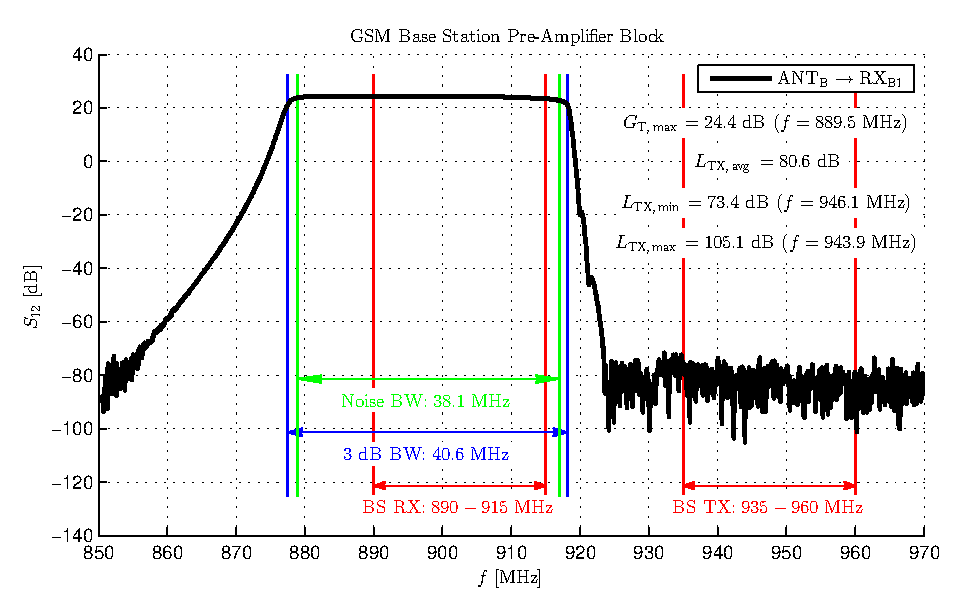
\epsfig{file=img/dpx.eps, width=\textwidth}
	\caption{Diplexer measurement.}
	\label{fig:dpx}
	\end{center}
	\vspace*{-12pt}
\end{figure}

The results suggest the diplexer insertion loss in the pass-band is approx. 1 dB, meaning the 
amp in the receive path (see Fig. \ref{fig:bs}) has a gain of roughly 30 dB. The total gain 
in the path is smaller than this due to the four-way power divider introducing 6 dB loss in 
each path (assuming ideal, equi-split divider). It is also possible there's a small gain 
compression in the VNA since the maximum VNA input power was roughly 4.4 dBm, but related 
information was omitted from the VNA specifications.

95 dB TX-RX diplexer isolation was required in the pre-study problem. Our measurements suggest 
that minimum isolation of 66 dB is achieved in the upper boundary of the RX band. Thus the 
95 dB requirement is not met. Nevertheless, one should not make hasty decisions based on a 
simplified calculation with more or less make-believe values. Also, effect of termination of 
the third port was not studied here. In our measurements, unused RX and TX ports were connected 
to the default operation setting, and ANT port was left open (as can be seen in Fig. \ref{fig:vna}).


\newpage
\section{Error estimates}

In this section, error estimates for the two types of measurements are presented.
The values presented here are only rough estimates based on literature (with more 
or less general cases) and their soundness in this case is somewhat questionable. 
In this section, we do not take human errors (see previous section) into account. 
It is just stated that systematic errors arising from the cables and connections 
are possible in measurement all measurements. Thus they are valid only for 
``correct'' measurements, and are more of the ``provided for completeness'' 
nature. Probabilities are not given due to the nature/basis of the estimation.


\subsection{Spectrum analyzer}

Each of the components inside the spectrum analyzer contributes to the total uncertainty, 
depending for example on the signal frequencies, amplitudes, and measurement settings. 
The Agilent (former HP, manufacturer of the used SA) has made available a document that 
specifies the different error sources, giving also rough estimates for some spectrum 
analyzers. According to the document \cite{sa}, the error estimates vary broadly among 
different analyzer models, giving worst case uncertainties exceeding $\pm 6$ dB. On the 
other hand, the document gives also representative values of amplitude uncertainties, 
which in our case yields about $\pm 1$ dB.

The second error source for the spectrum analyzer is the power marker reading. In 
each of the tasks, the spectrum analyzer was set to average 500 measurement points, 
which should average out most of the random errors. However, reading the power marker 
in the screen, there was a noticeable fluctuation in the shown power value. Based on the 
experience obtained during the measurements, the power marker error is estimated to be 
approximately $\pm 0.5$ dB.

In conclusion, the error estimates that can be taken into account numerically are 
the manufacturers representative value of approx. $\pm 1$ dB, and the power marker 
fluctuation of roughly $\pm 0.5$ dB. These uncorrelated errors may be summed to 
achieve the total uncertainty of the SA measurements of approx. $\pm 1.5$ dB. 

There is also the question of calibrating the spectrum analyzer properly with 
the time interval defined by the manufacturer. Agilent suggests to have the spectrum 
analyzer calibrated thoroughly once in a year, and quick-calibrated if there are 
changes operating environment \cite{sa2}. If the spectrum analyzer used in the 
measurements is not calibrated correctly, it is possible that the measurements are 
not reliable. In this case, the calibration is the most important error source, and 
the device should be calibrated correctly before estimating any other errors.


\subsection{Vector network analyzer}

For the VNA, different error sources and ways to cope with them are listed in the 
lecture slides discussing VNA measurements. The different sources are noise, 
cabling/connector repeatability, directivity, isolation, mismatch and environment 
induced drift. 

Noise and cabling/connector repeatability are random errors, which can be averaged 
out. In our case, only the noise was averaged, since we did not touch the cabling. 
Systematic errors arising directivity, isolation, and mismatch in this task were
for the most part neglected with a calibration. Before conducting measurements, 
the VNA is always calibrated using a standard calibration module. The calibration 
moves the reference planes to the connectors of the test cables, and somewhat 
cancels the systematic errors from the connectors and cables used in a specific 
measurement. Finally, the environment induced drift is not relevant, since the 
measurement was done inside a short time interval.

Rohde \& Schwarz provides specifications that describe the measurement uncertainty 
of the VNA in question in different frequency bands. For transmission measurements 
in the frequency range of 50 MHz to 3 GHz, accuracy for signal powers of $-50 \ldots 0$ 
dB is better than $0.2$ dB ($0.3$ dB for powers of $-50 \ldots {-70}$ dB) with 0 dBm 
transmit power. \cite{vna} The reader should note that these ranges was exceeded 
from both ends during the measurements (the measurement power range was roughly 
$-100 \ldots {+4}$ dBm). 

In conclusion, two things are assumed. First, calibration is assumed to cancel the 
systematic errors arising from cables and connectors. Second, random errors are 
cancelled with averaging. The manufacturer provides error estimates for the device 
itself, giving an error estimate of under $0.3$ dB that is mostly applicable in 
our case. The topics discussed in the last paragraph of the last subsection apply 
here to some extent to here as well.


\newpage
\section{Conclusions}

The purpose of the first laboratory assignment was to get familiar with the most 
common radio frequency measurement devices. This was done by measuring properties 
suchs as power level control, in-band and out-of-band amplitudes, and diplexer 
performance of a real-life GSM base station. In this report, results of these measurements
were presented and compared to GSM specifications. In addition, error sources 
and magnitudes were estimated.

The two most important error sources for the spectrum analyzer measurements are 
the power marker fluctuation and errors arising from the analyzer hardware. 
The fluctuation of the marker reading was estimated to be $\pm 0.5$ dB. The more 
difficult of the pair, errors originating in the analyzer, were estimated from 
the manufacturer's manual. The analyzer’s error was estimated to be $\pm 1$ dB. 
Together these uncorrelated errors give an error estimation of $\pm 1.5$ dB.

The vector network analyzer error estimations were easier, as the device is 
always calibrated using a specific calibration module. It was assumed that the 
calibration cancels the systematic errors arising from the measurement setup. In 
addition, the measurement was averaged in turn lowering the effect of random errors. 
Based on these assumptions, the measurement errors were estimated using the 
manufacturer’s manual, yielding better than 0.3 dB accuracy for the frequency 
range of interest.

The BS dynamic power control has 15 different power levels with a 2 dB step size. 
When comparing the measured results and assumed power levels in Table \ref{tbl:m1}, 
the difference is not more than $\pm 0.2$ dB. Given the estimated uncertainty of 
$\pm 1.5$ dB, it is difficult to evaluate the power control level performance. 
However, when excluding the uncertainty, each of the measurements agree well with 
the base station specifications. When taking this into account, it is relatively 
certain that the dynamic power control is working properly.

The results from the in-band output spectrum measurement are presented in Table 
\ref{tbl:m2}. The results are presented using the measured and given connection 
chain attenuations ($L = 43.1$ dB and $L = 36.0$ dB, respectively). While the 
results obtained using the measured attenuation do not pass the GSM specifications, 
the values obtained using the given attenuation pass the specification even with 
the estimated uncertainty of $\pm 1.5$ dB. Therefore, the result is that the 
base station passes the in-band GSM specifications. 

In subsection \ref{s:int}, the power levels of the single greatest interference in 
two bands (below and abode 1 GHz) was presented and compared against the GSM standard. 
In both bands, the measured values exceeded the specified limits, even when nominal 
attenuation was assumed. For the lower band, it was reasoned that the fault may be the 
nonlinearity of the SA (intermodulation perhaps) or the BS itself. In the upper band, 
the measured peak was created by the SA. Thus nothing definite can be said about the 
interference of the SA; it would require more measurements.

In the fourth measurement we were interested in the diplexer, the purpose of which 
is to separate the receiver and transmitter, while at the same time allowing a 
free route for the signal from the transmitter to the antenna and from the antenna 
to the receiver. In addition, there should be some gain in between the antenna 
and receiver. The measurement presented in Fig. \ref{fig:dpx} corresponds the 
aforementioned requirements. Diplexer separates the sides effectively, giving 
a minimum attenuation of $13.0$ dB in the ``no-man's land'' between the bands 
(66 dB at the upper edge of the RX band). The antenna-receiver path has a gain 
of $24.3$ dB, and the transmitter-antenna path attenuation is $-1.1$ dB. These 
results agree with the expected values.

For the most parts, the results presented here agree well with the expected 
results, even though there were some difficulties with the tasks that seemed 
so simple at a first glance. Dynamic downlink power control seems to work as 
advertised, and the base station seems to pass GSM specifications when it comes 
to the shape of in-band spectrum. Determining the interference characteristics 
would require more measurements. The diplexer measurements agree also well with the 
theory. 

In conclusion, we (re)familiarized ourselves with the measurement devices and got 
more knowledge about measurement devices nonlinearities for future reference.
It will be easier to perform measurements in both the upcoming assignments and in 
real-life as well. This in turn allows us to concentrate more on the actual results 
based on thorough and reliable measurements. However, defining different uncertainties 
presents still a challenge. Consequently, it should be taken into extra consideration 
when conducting RF measurements in the future.


\newpage
\section{Feedback}

The laboratory measurement was both interesting and educational 
even though it wasn't smooth sailing all the way. To be honest, 
it was more like the Bermuda triangle. There some minor 
issues and even some difficulties of the more major kind. Since 
we'd like no other students to go through such an ordeal, we'd like 
to give feedback. The following text will elaborate.

Let's start with the schedule. In our opinion its outright absurd/idiotic 
to have the lab in the last week of the semester, amidst the exams. On 
top of that, this final report is to be completed outside the 
curriculum, when everyone is spending their Christmas holiday 
most likely hundreds of miles away from Otaniemi. Thus we propose 
that either the lab (in its entirety) is held in November or postponed 
to January.

It seemed we were the ``try run'' and encountered issues the course 
staff was not properly prepared to deal with. It's somewhat like being 
handicapped against the other groups having the advantage. Also some 
topics we had our doubts about were not clarified as well as we'd hoped. 
These issues are covered in the next five paragraphs. Otherwise the 
course staff was pleasant to work with.

First, the course staff should be prepared for every foreseeable 
contingency by having their own try runs and going over the notes 
from previous years. How about making a checklist of sorts?

Second, having many years of experience from contact teaching and 
guiding laboratory measurements between us, we are safe say that 
students will not remember the theory given weeks ago in the heat 
of the moment. In some cases (freshmen) even 30 minutes is enough 
for a ``memory wipe.''

The theory needs to be tied to the task at hand. This can be done in 
numerous ways. One is to include a related problem (nonlinearity issues 
in this case) in the pre-study. Another is to print out the slides etc. 
to have the information available for students in the lab. This latter 
requires attention from the assistant.

Third, another go at the measurement would be more than welcome. It's 
way more demanding for a student to come up with the cause of a problem 
than to justify expected results. We'd reckon it would benefit the learning 
process as well. And in our case the time was running out, making the 
VNA measurements feel a bit too hasty.

Fourth, uncertainty is one of the not-so-clear topics. During the lectures, 
it was advertised as the most difficult aspect of a measurement and that 
its estimation requires experience above all. It's a daunting task at best, 
and to make it worse, we feel we were not given good enough ``tools'' to really
stand up to this challenged as first-timers. Determining the uncertainty in 
complex measurements (or in ``simple'' measurements with complex equipment) 
should be covered in more detail in the lectures or in the lab instructions. 
One could also print/point out the relevant information from the operators' 
manual. 

For easier VNA access, a USB-hub and a LCD-display would be great. 
The former costs around 5 euros and the latter can be found within 
the department, since a display too small for everyday use would do 
just fine. This kind of setup is used in the 
\textit{S-26.2300 Suurtaajuusmittaukset} course.

\newpage
\begin{thebibliography}{9}%\itemsep 7pt\parskip -5pt 

\bibitem{lab1} C.\ Icheln, S.\ Khanal, 
	\textit{GSM Transmitter laboratory assignment instructions},
	S-26.3120 Laboratory course in Radio Engineering course material.

\bibitem{sa} Agilent, Spectrum Analysis Basics, Application Note 150. 
	Available online at \url{http://cp.literature.agilent.com/litweb/pdf/5952-0292.pdf} 
	[Retrieved: Jan 2nd, 2014].
	
\bibitem{sa2} Agilent, 8590 Series Analyzers Calibration Guide.
	Available online at \url{http://cp.literature.agilent.com/litweb/pdf/08594-90106.pdf}
	[Retrieved: Jan 2nd, 2014].
	
\bibitem{vna} R\&S ZVL Vector Network Analyzer Specifications, 
	Version 06.00, Dec 2008. 
	Available online at \url{http://www.upc.edu/pct/documents_equipament/d_160_id-655-2.pdf} 
	[Retrieved: Jan 2nd, 2014].


%\bibitem{pozar} D.\ M.\ Pozar, 
%	\textit{Microwave Engineering}, 
%	J.\ Wiley \& Sons, 4th Edition, 2012. 
%	ISBN: 978-0-470-63155-3.
	
%\bibitem{gains} J.\ C.\ Logan, J.\ W.\ Rockway, 
%	``Dipole and Monopole Antenna Gain and Effective Area for Communication Formulas.''
%	Available online at \url{www.dtic.mil/cgi-bin/GetTRDoc?AD=ADA332891}
%	[Retrieved: November 25, 2013].

%\bibitem{parts} M.\ Steer, 
%	\textit{Microwave and RF Design -- A Systems Approach}, 
%	SciTech Publishing, 2010. 
%	ISBN: 978-1-891-12188-3.
	
%\bibitem{iet} R.\ J.\ Collier, A.\ D.\ Skinner (editors), 
%	\textit{Microwave Measurements}, 
%	The Institution of Engineering and Technology, 3rd Edition, 2007. 
%	ISBN: 978-0-86341-735-1.

\end{thebibliography}

\end{document}
